\documentclass[12pt]{article}
\usepackage[utf8]{inputenc}
\usepackage[serbian]{babel} % Podrška za srpski jezik i gramatiku
\usepackage{amsmath} % Paket za matematičke komande
\usepackage{graphicx} % Omogućava ubacivanje slika

\title{Seminarski rad: Osnove matematičkog modeliranja}
\author{Tvoje Ime i Prezime}
\date{\today}

\begin{document}
\maketitle

\section{Uvod i postavka matematičkog modela}

U ovom seminarskom radu proučavamo dinamiku populacije uličnih pasa u zatvorenom staništu pod uticajem kontrole od strane šinterske službe. Modeliranje vršimo u kontinualnom vremenu, gde vreme $t$ merimo u godinama, a stanje populacije posmatramo preko gustine populacije $x(t)$, koja predstavlja broj jedinki po kvadratnom kilometru ($\text{jedinki/km}^2$).

\subsection{Pretpostavke modela}
Pre same matematičke formulacije, definišemo osnovne biološke i ekološke pretpostavke pod kojima razvijeni model važi:
\begin{itemize}
    \item \textbf{Zatvorenost staništa:} Pretpostavlja se da nema migracija, odnosno da su imigracija (doseljavanje) i emigracija (odseljavanje) pasa zanemarljive.
    \item \textbf{Ograničenost resursa:} Resursi u okruženju (hrana, sklonište, prostor) su konačni. Maksimalni kapacitet sredine koji stanište može prirodno da podrži iznosi $K = 250 \, \text{jedinki/km}^2$.
    \item \textbf{Logistički rast:} U odsustvu spoljašnjih faktora, populacija se razmnožava po logističkom zakonu. Za malu gustinu populacije, konstantna stopa nataliteta iznosi $b = 0.34$, a stopa mortaliteta $d = 0.12$ na godišnjem nivou.
    \item \textbf{Kontinuirana eutanazija:} Šinterska služba deluje neprekidno tokom godine i uklanja (hvata i eutanazira) konstantan procenat $\epsilon$ od trenutnog broja postojećih pasa. U daljem radu, parametar $\epsilon$ posmatramo kao udeo ($\epsilon \in [0,1]$).
\end{itemize}

\subsection{Formulacija diferencijalne jednačine}
Inherentna (unutrašnja) stopa rasta populacije u uslovima neograničenih resursa predstavlja razliku između stope nataliteta i stope prirodnog mortaliteta:
$$ r = b - d = 0.34 - 0.12 = 0.22 \, \text{godina}^{-1} $$

Klasičan logistički model rasta populacije bez uticaja čoveka opisan je diferencijalnom jednačinom:
$$ \frac{dx}{dt} = r \cdot x \left(1 - \frac{x}{K}\right) $$

Uvođenjem stope eutanazije, koja direktno zavisi od trenutne gustine populacije $x(t)$, dobijamo konačnu nelinearnu običnu diferencijalnu jednačinu prvog reda koja opisuje naš model:
\begin{equation}
\frac{dx}{dt} = r \cdot x \left(1 - \frac{x}{K}\right) - \epsilon \cdot x
\end{equation}

Sređivanjem desne strane jednačine (1), model možemo zapisati u ekvivalentnom obliku pogodnom za analizu:
\begin{equation}
\frac{dx}{dt} = (r - \epsilon)x - \frac{r}{K}x^2
\end{equation}


\section{Analitičko rešenje diferencijalne jednačine}

Kako bismo precizno analizirali ponašanje populacije uličnih pasa kroz vreme, jednačinu (2) rešićemo egzaktno (analitički). Uočavamo da je jednačina nelinearna obična diferencijalna jednačina prvog reda koja se može rešiti metodom razdvajanja promenljivih:
$$ \frac{dx}{dt} = x \left( (r - \epsilon) - \frac{r}{K}x \right) $$

Razdvajanjem promenljivih, pod pretpostavkom da je desna strana različita od nule, dobijamo:
\begin{equation}
\frac{dx}{x \left( (r - \epsilon) - \frac{r}{K}x \right)} = dt
\end{equation}

Integralićemo levu stranu jednačine (3) korišćenjem metode razlaganja podintegralne funkcije na proste razlomke:
$$ \frac{1}{x \left( (r - \epsilon) - \frac{r}{K}x \right)} = \frac{A_0}{x} + \frac{B_0}{(r - \epsilon) - \frac{r}{K}x} $$

Množenjem ove relacije sa zajedničkim imeniocem dobijamo identitet po $x$:
$$ 1 = A_0(r - \epsilon) + \left( B_0 - A_0\frac{r}{K} \right)x $$

Izjednačavanjem koeficijenata uz odgovarajuće stepene od $x$, dobijamo sistem jednačina iz kog sledi da je $A_0 = \frac{1}{r - \epsilon}$ i $B_0 = \frac{r}{K(r - \epsilon)}$. Sređivanjem integrala, integracija daje:
$$ \frac{1}{r - \epsilon} \left( \ln|x| - \ln\left|(r - \epsilon) - \frac{r}{K}x\right| \right) = t + C_1 $$

Množenjem cele jednačine sa $(r - \epsilon)$ i primenom osobina logaritma, a potom i eksponenciranjem obe strane jednačine, oslobađamo se logaritma:
\begin{equation}
\frac{x}{(r - \epsilon) - \frac{r}{K}x} = C \cdot e^{(r - \epsilon)t}
\end{equation}
gde je $C$ integraciona konstanta. Neka je u početnom trenutku $t=0$ poznata početna gustina populacije $x(0) = x_0$. Zamenom ovih vrednosti u jednačinu (4) određujemo konstantu $C$:
$$ C = \frac{x_0}{(r - \epsilon) - \frac{r}{K}x_0} $$

Iz jednačine (4) eksplicitno izražavamo rešenje $x(t)$ po vremenu i nakon sređivanja dobijamo \textbf{konačno analitičko rešenje}:
\begin{equation}
x(t) = \frac{(r - \epsilon)x_0}{\frac{r}{K}x_0 + \left(r - \epsilon - \frac{r}{K}x_0\right)e^{-(r - \epsilon)t}}
\end{equation}


\section{Diskusija rešenja za zadate stope eutanazije}

Kvalitativna analiza modela i stabilnost populacije zavise od stacionarnih stanja (tačaka ravnoteže) koje dobijamo izjednačavanjem desne strane jednačine (2) sa nulom:
$$ x \left( (r - \epsilon) - \frac{r}{K}x \right) = 0 \implies x_1^* = 0, \quad x_2^* = K\left(1 - \frac{\epsilon}{r}\right) $$

U zavisnosti od vrednosti parametra $\epsilon$ koji kontroliše šinterska služba, razlikujemo dva suštinski različita biološka scenarija, što potvrđujemo i numeričkim eksperimentom u MATLAB-u (pomoću funkcije \texttt{ode45}), uz pretpostavljenu početnu gustinu populacije $x_0 = 150 \, \text{jedinki/km}^2$ u periodu od 50 godina.

\begin{figure}[htbp]
    \centering
    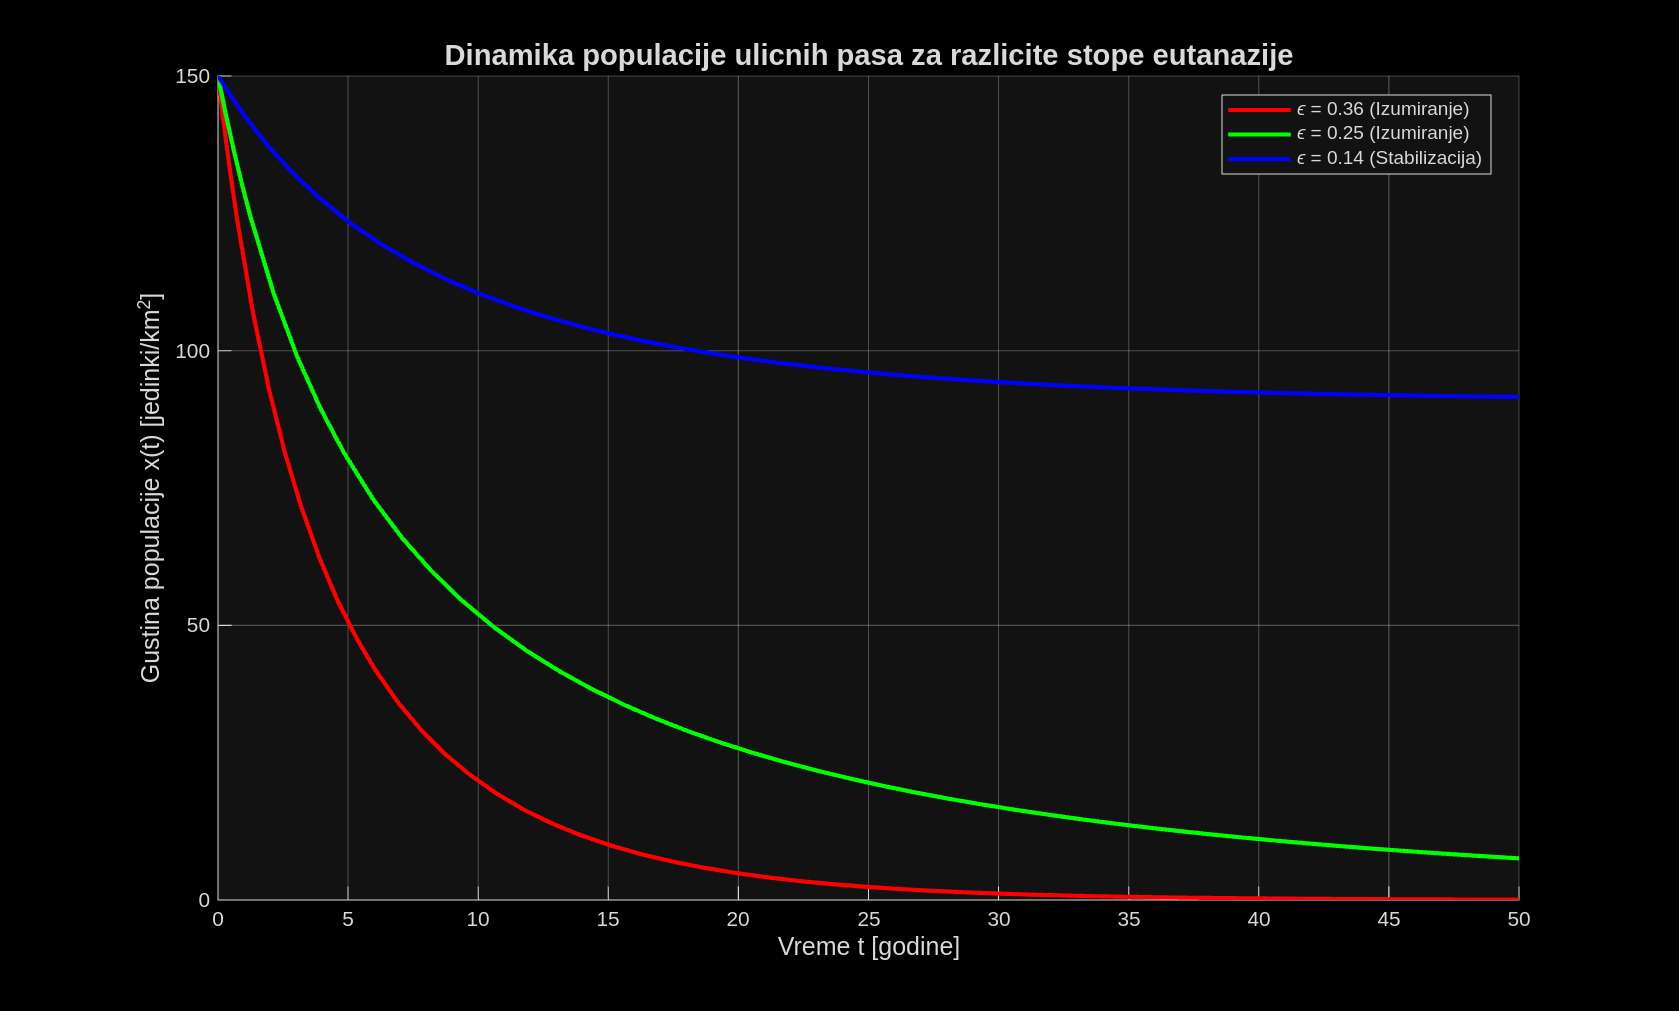
\includegraphics[width=0.8\textwidth]{grafik_pasa.png}
    \caption{Simulacija kretanja gustine populacije uličnih pasa kroz vreme bez spoljašnjeg priliva.}
    \label{fig:grafik_pasa}
\end{figure}

Na osnovu teorijske analize i generisanog grafika sa slike \ref{fig:grafik_pasa}, diskutujemo sledeće slučajeve:
\begin{enumerate}
    \item \textbf{Slučaj $\epsilon = 0.36$ i $\epsilon = 0.25$:} Stopa eutanazije je veća od stope rasta ($\epsilon > r = 0.22$). Član $r - \epsilon$ je negativan, pa u limitu $t \to \infty$ populacija teži tački $x_1^* = 0$. Crvena linija ($\epsilon = 0.36$) opada najbrže i dovodi do izumiranja oko 25. godine, dok zelena linija ($\epsilon = 0.25$) sporije teži nuli.
    \item \textbf{Slučaj $\epsilon = 0.14$:} Stopa eutanazije je manja od stope priraštaja ($\epsilon < r$). Pošto je $r - \epsilon > 0$, populacija opstaje i stabilizuje se na nivou: $x_2^* = 250 \cdot (1 - \frac{0.14}{0.22}) \approx 90.91 \, \text{jedinki/km}^2$, što plava linija i potvrđuje.
\end{enumerate}


\section{Prošireni model sa prilivom napuštenih pasa}

U ovom delu rada proširujemo osnovni model uvođenjem realistične pretpostavke o neodgovornom vlasništvu. Pretpostavlja se da svake godine konstantan broj $A$ napuštenih pasa (po $\text{km}^2$) biva izbačen na ulicu i time oni postaju deo populacije uličnih pasa. 

Nova diferencijalna jednačina koja opisuje ovaj proces ima oblik:
\begin{equation}
\frac{dx}{dt} = r \cdot x \left(1 - \frac{x}{K}\right) - \epsilon \cdot x + A
\end{equation}
Sređivanjem izraza po opadajućim stepenima promenljive $x$, dobijamo kvadratnu formu sa desne strane:
\begin{equation}
\frac{dx}{dt} = -\frac{r}{K}x^2 + (r - \epsilon)x + A
\end{equation}

\subsection{Stabilna stanja proširenog modela}
Tačke ravnoteže dobijamo rešavanjem kvadratne jednačine $-\frac{r}{K}x^2 + (r - \epsilon)x + A = 0$, odnosno:
$$ \frac{r}{K}x^2 - (r - \epsilon)x - A = 0 $$

Korišćenjem kvadratne formule, rešenja za tačke ravnoteže su:
\begin{equation}
x_{1,2}^* = \frac{(r - \epsilon) \pm \sqrt{(r - \epsilon)^2 + 4 \frac{r}{K}A}}{2\frac{r}{K}}
\end{equation}

Budući da su parametri $r, K, A > 0$, diskriminanta pod korenom $D = (r - \epsilon)^2 + 4 \frac{r}{K}A$ je strogo pozitivna za svako $\epsilon$, što znači da uvek postoje dva realna rešenja. Fizički i biološki smisao ima samo pozitivno rešenje:
\begin{equation}
x^* = \frac{(r - \epsilon) + \sqrt{(r - \epsilon)^2 + 4 \frac{r}{K}A}}{2\frac{r}{K}}
\end{equation}

Uočavamo ključnu promenu: \textbf{Tačka ravnoteže $x^* = 0$ više ne postoji kao rešenje sistema dokle god je $A > 0$}. To znači da se ulični psi više ne mogu u potpunosti istrebiti na duži rok, jer čak i ako u nekom trenutku broj pasa spadne na nulu, konstantan priliv $A$ odmah ponovo pokreće rast populacije.

\subsection{Numerički eksperiment i grafički prikaz}
Da bismo vizuelizovali ponašanje proširenog modela, sprovodimo numerički eksperiment u MATLAB-u uzimajući pretpostavljenu vrednost priliva $A = 10 \, \text{pasa/km}^2$ godišnje, dok ostali parametri i početni uslov ($x_0 = 150$) ostaju isti.

\begin{figure}[htbp]
    \centering
    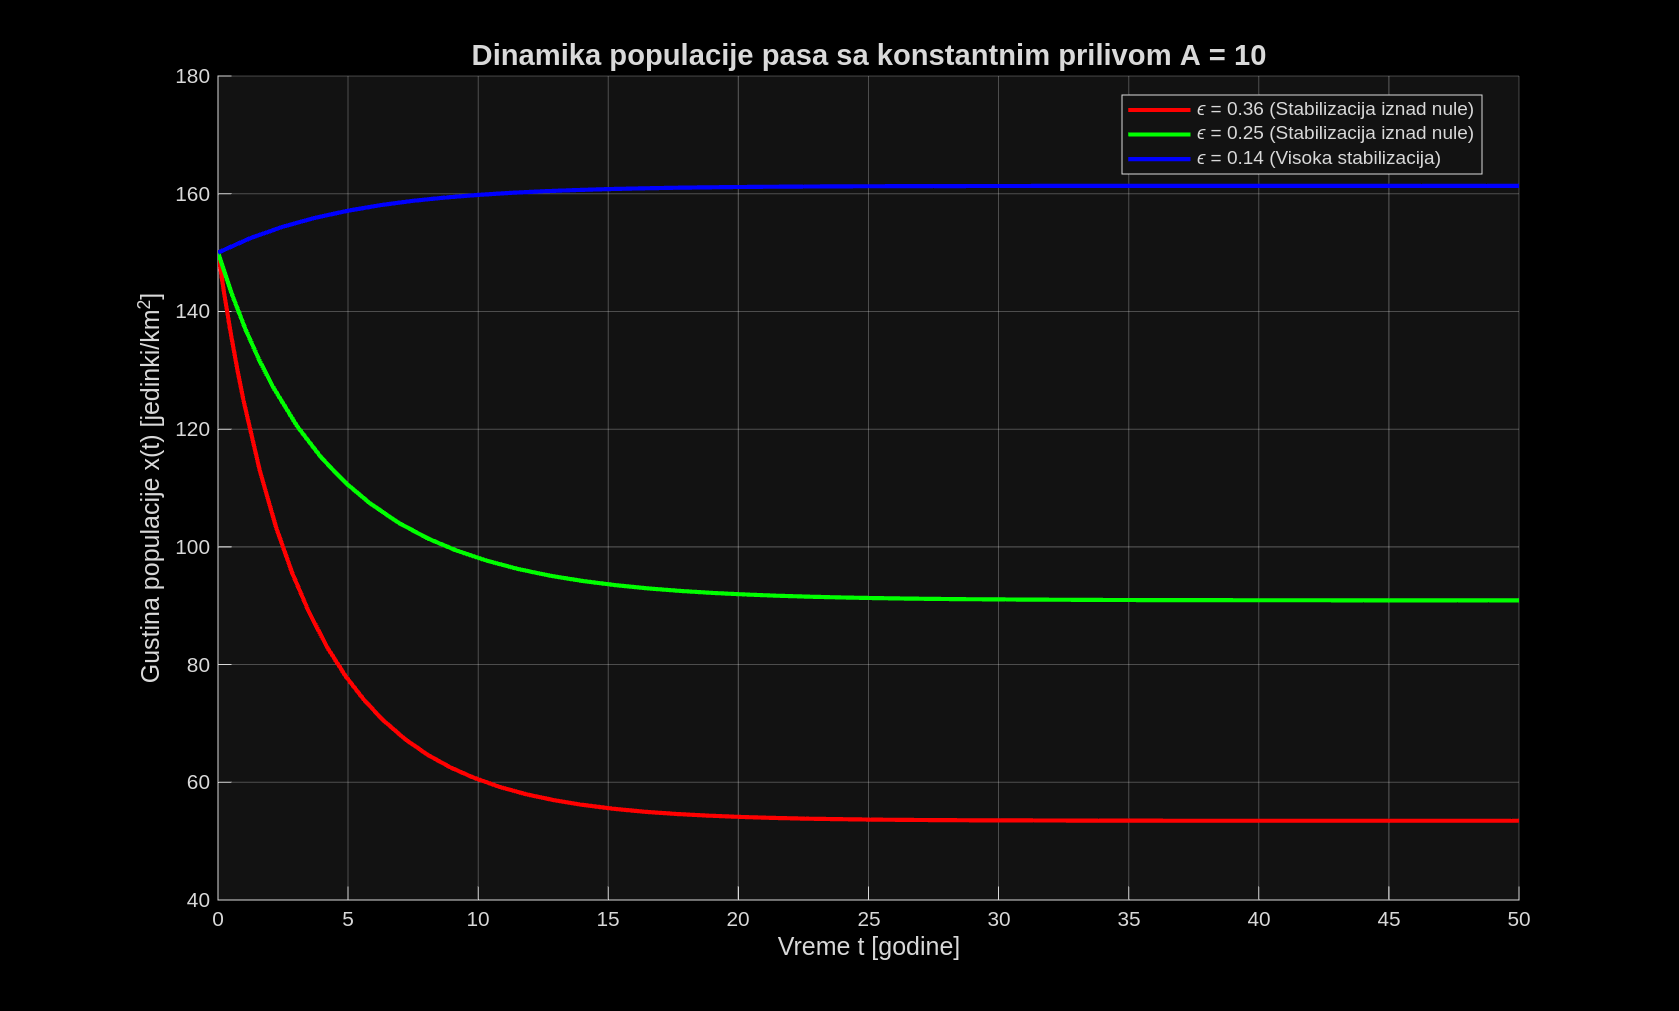
\includegraphics[width=0.8\textwidth]{grafik_napusteni.png}
    \caption{Dinamika populacije sa konstantnim godišnjim prilivom napuštenih pasa $A = 10$.}
    \label{fig:grafik_napusteni}
\end{figure}

Na osnovu slike \ref{fig:grafik_napusteni} uočavamo sledeće:
\begin{itemize}
    \item Za $\epsilon = 0.36$ (crvena linija) i $\epsilon = 0.25$ (zelena linija), iako je intenzitet eutanazije veći od prirodnog priraštaja, populacija ne izumire. Krive asimptotski prilaze novoj stabilnoj vrednosti koja je strogo veća od nule. Zamenom vrednosti u formulu (9) dobijamo da se za $\epsilon=0.36$ populacija stabilizuje na oko $54 \, \text{jedinki/km}^2$.
    \item Za $\epsilon = 0.14$ (plava linija), populacija se stabilizuje na značajno višem nivou nego u prvom delu rada (oko $162 \, \text{jedinki/km}^2$), jer se na prirodni priraštaj konstantno dodaju i napušteni psi vlasnika.
\end{itemize}

\section{Zaključak}
Kroz ovaj rad smo pokazali moć matematičkog modeliranja u ekologiji i upravljanju komunalnim problemima. Dok je u idealnom slučaju (bez neodgovornog vlasništva) agresivna eutanazija mogla dovesti do potpunog uklanjanja problema uličnih pasa, u realnom scenariju gde postoji konstantan priliv $A$, istrebljenje je nemoguće. Jedina održiva strategija jeste kombinacija kontrole populacije i drastičnog smanjenja parametra $A$ kroz zakonske regulative i čipovanje kućnih ljubimaca.

\newpage
\begin{thebibliography}{9}
\bibitem{logisticki} 
J. D. Murray, \textit{Mathematical Biology: I. An Introduction}, Springer-Verlag, New York, 2002.
\bibitem{diferencijalne}
M. Braun, \textit{Differential Equations and Their Applications}, Springer, 1993.
\bibitem{matlab}
The MathWorks Inc., \textit{MATLAB and Simulink for Modeling and Simulation}, R2025b.
\end{thebibliography}

\end{document}